\subsection{Construction Time Experiments} 

To evaluate the performance of the implemented algorithms, we conducted a series of experiments on randomly generated trees, with sizes ranging from 100 to 900,000 nodes. For each tree, we executed the construction algorithms 10 times, recording the average execution time for both the linear \textsc{PathSort} algorithm and the Naive Sort algorithm used for constructing the XBWT.
By ``Naive Sort'', we refer to a straightforward approach that first precomputes all the upward paths in the tree and then sorts them using a standard sorting algorithm. This method contrasts with \textsc{PathSort}, which is specifically designed to achieve linear time complexity in path sorting.
This approach enabled us to compare their performance across various tree sizes and evaluate their scalability.

From the results shown in Table \cref{tab:experiments}, we can draw several conclusions about the performance of the \textsc{PathSort} algorithm compared to the Naive Sort algorithm.

The \textsc{PathSort} algorithm consistently outperforms the Naive Sort algorithm in terms of execution time, especially as the number of nodes increases. For smaller trees, the difference in execution time between the two algorithms is minimal. However, as the number of nodes grows, the \textsc{PathSort} algorithm demonstrates significantly better scalability. For instance, with 900,000 nodes, the \textsc{PathSort} algorithm takes 8.51 seconds, whereas the Naive Sort algorithm takes 34.2 seconds, giving a speedup of more than $4\times$. A visual representation of the results can be seen in \cref{fig:xbwt_exp_plots} where both the time comparison and the speedup are shown.

\begin{table}[h]
    \centering
    \begin{tabular}{|r|r||r|r|}
        \hline
        \textbf{\# Nodes} & \textbf{Depth} & \textbf{Naive Sort (s)} & \textbf{\textsc{PathSort} (s)} \\
        \hline
            100 &    22 &  0.001 & 0.002 \\
            500 &    45 &  0.002 & 0.004 \\
          1,000 &    74 &  0.003 & 0.006 \\
          5,000 &   175 &  0.015 & 0.028 \\
         10,000 &   288 &  0.053 & 0.056 \\
         50,000 &   486 &  0.350 & 0.310 \\
        100,000 &   754 &  1.250 & 0.690 \\
        500,000 & 2,246 & 16.460 & 4.700 \\
        900,000 & 2,658 & 34.200 & 8.510 \\
        \hline
    \end{tabular}
    \caption{Performance comparison of the execution times for the Naive Sort and \textsc{PathSort} algorithms on randomly generated trees of varying sizes.}
    \label{tab:experiments}
\end{table}

\begin{figure}[H]
    \centering
    \begin{subfigure}[b]{0.48\textwidth}
        \centering
        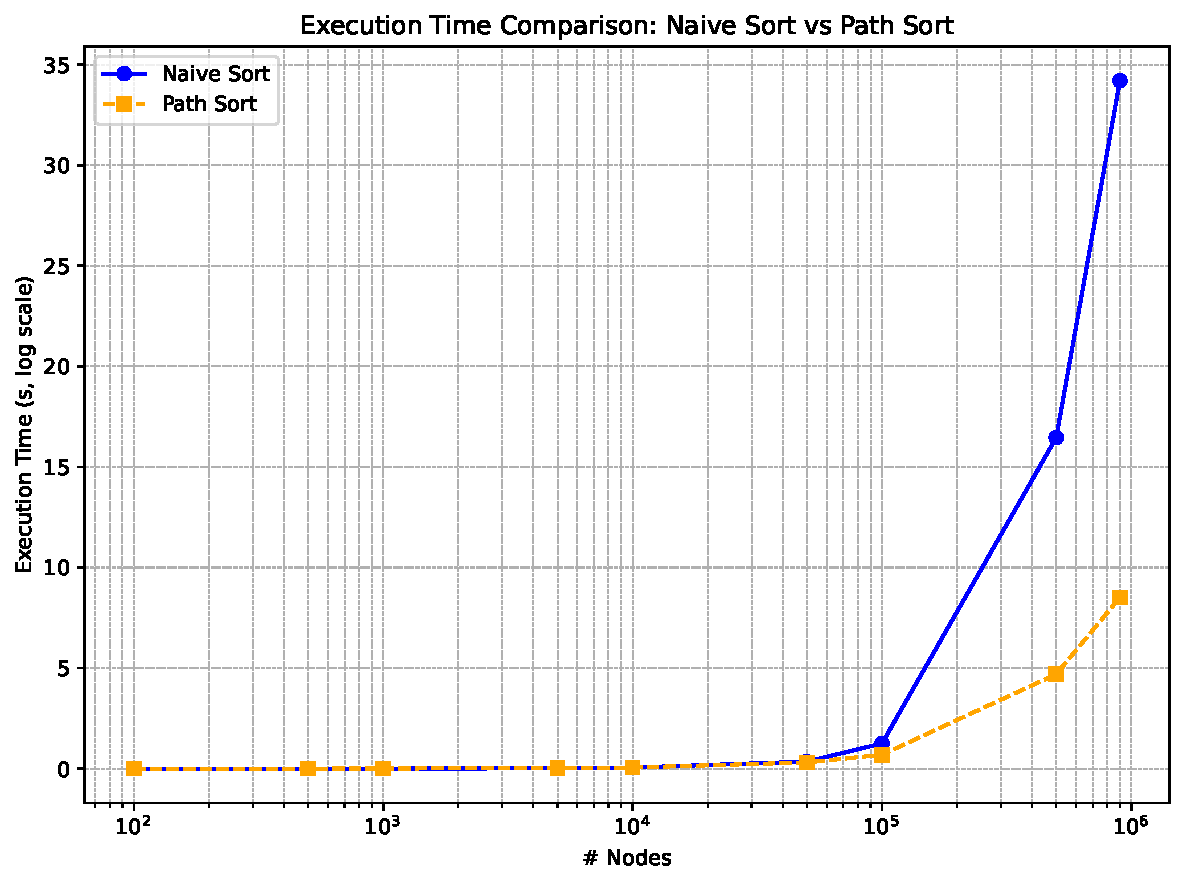
\includegraphics[width=\textwidth]{"Immagini/execution_time_comparison.pdf"}
        \caption{Time Comparison}
        \label{fig:time_comparison}
    \end{subfigure}
    \hfill %
    \begin{subfigure}[b]{0.48\textwidth}
        \centering
        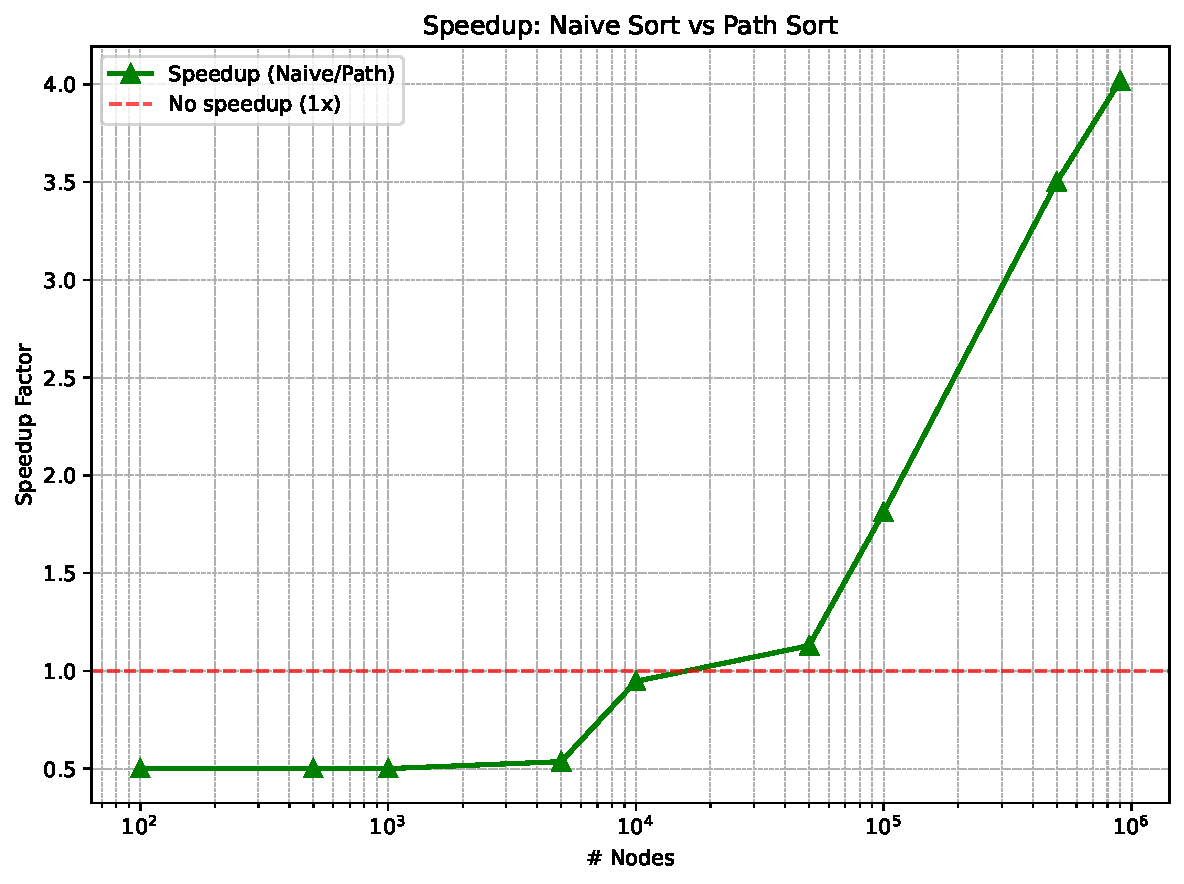
\includegraphics[width=\textwidth]{"Immagini/speedup_comparison.pdf"}
        \caption{Speedup}
        \label{fig:speedup}
    \end{subfigure}
    \caption{Time comparison and speedup plots for the experiments in \cref{tab:experiments}. Image (a) shows \textsc{PathSort} time in seconds (yellow dashed line) vs. Naive Sort time (blue line). Image (b) shows the speedup of \textsc{PathSort} over Naive Sort. The area below the red dashed line indicates points where the speedup is less than or equal to 1, representing no improvement of \textsc{PathSort} over Naive Sort.}
    \label{fig:xbwt_exp_plots}
\end{figure}

\begin{comment}
\subsubsection{Space Analysis}
To evaluate the space savings achieved through XBWT compression, we conducted experiments on the same set of randomly generated trees used for the construction performance tests. For each tree, we compared the memory usage (in bytes) of three representations: the plain tree, the uncompressed XBWT, and the compressed XBWT.

The plain tree representation consists of the simple balanced parentheses encoding of the tree structure combined with the edge labels. For example, for the tree in \cref{fig:example_tree,tab:xbwt_example}, the plain tree representation would be:

\texttt{(A(B(D(a))(a)(E(b)))(C(D(c))(b)(D(c)))(B(D(b))))}.

By \emph{uncompressed XBWT}, we refer to the XBWT arrays $S_{\text{last}}$ and $S_{\alpha}$ (including the additional bit) stored without any compression. Specifically, $S_{\text{last}}$ is represented as a plain bitvector (\texttt{sdsl::bit\_vector}), and $S_{\alpha}$ is stored as a wavelet tree (\texttt{sdsl::wt\_int}) with plain bitvectors (\texttt{sdsl::bit\_vector}). In contrast, the \emph{compressed XBWT} representation stores $S_{\text{last}}$ and $S_{A}$ as compressed RRR bitvectors (\texttt{sdsl::rrr\_vector}), and $S_{\alpha}$ as a wavelet tree with RRR bitvectors, as described in the previous chapter.

\cref{tab:experiments_2} reports the sizes (in bytes) for each representation of the trees across different sizes. The last column highlights the space savings achieved by the compressed XBWT compared to the plain tree representation, expressed as a percentage. These results illustrate the substantial space reductions achieved through compression, especially as the tree size increases.

%\alessio{Oltre ai punti di prima, metti la percentuale anche per UXBWT, magari non come un'altra colonna ma metti tra parentesi. Te lo faccio sulle prime righe per la C.XBWT. Se ti piace, ricorda di spiegare cosa sono i numeri tra parentesi nella descrizione.}
\begin{table}[ht]
    \centering
    \begin{tabular}{|r||r|r|r|}
        \hline
        \textbf{\# Nodes} & \textbf{Plain tree} & \textbf{U. XBWT} & \textbf{C. XBWT} \\
        \hline
            100 &       390 &       424 &       496 \color{gray}{(-27.18\%)}\\
            500 &     2,390 &     1,112 &     1,136 ~\color{gray}{(52.47\%)} \\
          1,000 &     4,890 &     2,242 &     2,056 ~\color{gray}{(57.96\%)} \\
          5,000 &    28,890 &    12,911 &    10,400 ~\color{gray}{(64.00\%)} \\
         10,000 &    58,890 &    45,625 &    21,848 ~\color{gray}{(62.90\%)} \\
         50,000 &   338,890 &   175,146 &   123,216 ~\color{gray}{(63.64\%)} \\
        100,000 &   688,890 &   349,478 &   259,376 ~\color{gray}{(62.35\%)} \\
        500,000 & 3,888,890 & 1,850,850 & 1,451,570 ~\color{gray}{(62.67\%)} \\
        900,000 & 7,088,890 & 3,480,190 & 2,718,570 ~\color{gray}{(61.65\%)} \\
        \hline
    \end{tabular}
    \caption{Space analysis of the XBWT. The first column represents the number of nodes, the others the bytes used by each representation.
    ``Plain tree'' is the size of the tree in the simple balanced parenthesis representation plus the edge labels, ``U. XBWT'' is the size of the uncompressed XBWT, and ``C. XBWT'' is the size of the compressed XBWT.
    Gray numbers between parentheses represent the improvement relative to the plain tree representation.}
    \label{tab:experiments_2}
\end{table}

For small trees, the compressed XBWT does not always provide immediate savings due to the overhead of succinct data structures. For instance, for 100 nodes, the compressed representation is larger than the plain tree, showing a \(-27.18\%\) increase in space. However, as the number of nodes increases, the compression becomes more effective, achieving savings of over 60\% for large trees.

The space reduction becomes particularly evident for trees with more than 500 nodes. These results confirm that the compressed XBWT provides a scalable and space-efficient alternative for storing and indexing labeled trees. The efficiency gains are particularly beneficial for applications requiring large-scale tree processing, such as bioinformatics and text indexing.
\end{comment}
